
\lettrine[lines=3]{T}{}he L-system at its core is a formal grammar made up of an \textit{alphabet} of characters which are concatenated together into collections of symbols, called strings. The L-system describes a starting string called the \textit{axiom}, and a set of production rules. For each rewriting step the production rules determine whether a symbol within a string should be rewritten with another symbol or string. Each symbol within the \textit{axiom} is matched against the production rules. If a match is found, the symbol within the axiom is replaced with a predecessor string described by the production rule. This process is carried out for each symbol in the \textit{axiom}. The resulting string created by the rewriting process then becomes the axiom, which can then be rewritten once again. This process of rewriting using production rules is the mechanism for generating a structure of states that obay the production rules, similar to that of a context-free grammar. Essentially the symbols represent a particular state of the system, and the production rules decide whether that state should transition based on a certain criteria, and what the next state should be. 

This chapter will discuss a number of different types of L-systems, as well as their features and limitations. It will focus on the mechanics behind the rewriting system and different techniques that can be used to better represent plant-life as an L-system. In order to provide sufficient background, this chapter will also touch briefly on how the resulting strings generated by the L-system can be interpreted. The interpretation of an L-system is a separate system to the L-system, however, it is important to note that the L-system itself has no concept of what it is trying to represent, it is simply a string rewriting system. The L-systems interpretation is left up to a separate system, responsible for interpreting the resulting string to create a suitable representation for that problem domain. For instance, the symbols for a L-system trying to represent a tree, may be interpreted very differently to the symbols trying to represent music, however, the L-systems may be identical. Although the interpreter is not neccessarily part of the L-system it is an important to understand the reliance of the L-system on the string interpreter. The string interpreter will be in great detail in chapter \ref{interpreter implementation}.


A well-known biologist, Aristid Lindenmayer, started work on the Lindenmayer System or L-system in 1968, he sought to create a new method of simulating the growth in multicellular orgamisms such as algae and bacteria \cite{lindenmayer1968mathematical}. He later defined a formal grammar for simulating multicelular growth which he called the 0L-system \cite {lindenmayer1971developmental}. In the last twenty years, the concept has been adapted to be used to describe larger organisms such as plants and trees as well as other non organic structures like music \cite{worth2005growing}. There has also been studies to try to use an L-system as a method of creating and controlling growth of a connectionist model to represent human perception and cognition \cite{vaario1991connectionist}. Similarly, K{\'o}kai et al. (1999) have created a method of using a parametric L-system to describe the human retina, this can be combined with evolutionary operators and be applied to patients with diabetes who are being monitored \cite{kokai1999parametric}.


\section{Simple DOL-system} \label{Simple DOL-systems}

According to Prusinkiewicz and Hanan the most simple type of L-system is known as the D0L-system. The term 'D0L system' abbreviates 'Deterministic Lindenmayer system with zero-sided interactions'. It is deterministic because each symbol has an associated production rule and there is no randomness in determining which rule should be chosen for rewriting. A zero-sided interaction refers to the multicellular representation of an L-system, where each symbol refers to a type of cell, each cell does not account for the state of its direct neighbouring cells, making it zero-sided. There are three major parts to a D0L system. Firstly there is a finite set of symbols known as the \textit{alphabet}, a starting string or \textit{axiom} and the state transition rules \textit{production rules}. The alphabet is a set of characters which represent a state in a system. The axiom is the starting point of the system which contains one or more characters from the alphabet. The transition rules dictate whether a state should remain the same, or transition into a different state, or even disappear completely. \cite{prusinkiewicz2013lindenmayer}. 

The DOL-system was originally created to serve as a context-free grammar, to represent the development of multicellular organisms. The DOL-system shown in \ref{DOL-system example} below, is an example formulated by Prusinkiwicz and Lindenmayer to simulate Anabaena Catenula which is a type of filamentous cyanobacteria which exists in plankton. According to Prusinkiewicz and Lindenmayer \say{Under a microscope, the filaments appear as a sequence of cylinders of various lengths, with $a$-type cells longer than $b$-type cells. The subscript $l$ and $r$ indicate cell polarity, specifying the positions in which daughter cells of type $a$ and $b$ will be produced.} \cite{prusinkiewicz2012algorithmic}.

\begin{equation} \label{DOL-system example}
\begin{aligned}
	&\omega~~ : a_r \\
	&p_1~ :  a_r~ \rightarrow~ a_l b_r\\
	&p_2~ :  a_l~ \rightarrow~ b_l a_r\\
	&p_3~ :  b_r~ \rightarrow~ a_r\\
	&p_4~ :  b_l~ \rightarrow~ a_l\\
\end{aligned}
\end{equation}

\noindent
With the definition above, the : symbol separates the axiom and production names from their values, furthermore the $\rightarrow$ can be verbalised as "is replaced by" or "rewritten with". The DOL-system states that $w~ :~ a_r$, where the symbol $w$ signifies that what follows is the axiom, therefore, the starting point is the cell $a_r$. The production rules then follow and are $p1, p2, p3$ and $p4$. In production rule 1 ($p1$) the cell $a_r$ will be rewritten with cells $a_l b_r$. Production rule $p2$ states that $a_l$ will be rewritten with cells $b_l a_r$. Production rule $p3$ states $b_r$ will rewritten with cell $a_r$ and finally production rule 4 ($p4$), states that $b_l$ will be rewritten with cell $a_l$. In order to simulate Anabaena catenula we require these four rewriting rules, as there are four types of state transitions. The resultant strings for five generations of the rewritting process can be seen in \ref{DOL-system result string} below: 

\begin{equation} \label{DOL-system result string}
\begin{aligned}
	& G_0~ :~ a_r \\
	& G_1~ :~ a_l b_r \\
	& G_2~ :~ b_l a_r a_r \\
	& G_3~ :~ a_l a_l b_r a_l b_r \\
	& G_4~ :~ b_l a_r b_l a_r a_r b_l a_r a_r \\
	& G_5~ :~ a_l a_l b_r a_l a_l b_r a_l b_r a_l a_l b_r a_l b_r \\
\end{aligned}
\end{equation}

\noindent
During the rewriting process, generation zero ($G_0$) is the axiom. In subsequent generations the resultant string of the previous generation is taken and each symbol in the string is compared to the production rules. If they match the production rule the symbol is rewritten with the successor symbol or string, which is specified by the production rule. For instance, the previous generation for $G_1$ is $G_0$ and the resultant string is for $G_0$ is $a_r$, the first symbol in this resultant string is compared with the production rules. In this case $a_r$ matches rule $p1$ with the rule being $p1~ :~ a_r~ \rightarrow~ a_l b_r$ and therefore, $a_r$ is rewritten with $a_l b_r$. The resultant string of $G_0$ only has one symbol, so it can be concluded that the string of $G_1$ is $a_l b_r$, this string is stored for the next rewriting step and is later rewritten to produce generation two and so on, until the desired number of generations is reached.

The D0L-system is very simple and minimalist in design, which comes with some limitations. The D0L-system production rules merely state that if the symbol matches the production rule, then that symbol will be rewritten. Often this is not the case, there may be some other conditions that may need to be checked before it can be concluded that a rewrite should take place. Furthermore, the symbols within a D0L-system does not supply much information. For instance, how does the D0L-system indicate how many times a given string has been rewritten? The D0L-system is also deterministic, meaning that there is no randomness the rewriting process, and therefore, it will always yield the same result with no variation. This can be seen as a limitation as variation within the system may be a seen as a good thing, such as variation within the branching structure of plants. 

\section{Interpreting the DOL-system String} \label{Interpreting DOL-system}

Section \ref{Simple DOL-systems} outlined a simple type of L-system known as the DOL-system. This type of L-system specifies an alphabet, an axiom and a set of production rules. This allows the representation of a problem as a set of states. The production rules can express valid state transitions, eventually produces a resulting string of symbols that obey the L-systems production rules. This functionality is powerful; however, the L-system's symbols are only useful if they represent some meaning. Furthermore, the L-system does not supply this meaning, each symbol's meaning is interpreted after the rewriting process by the interpreter. Due to this, there are two separate systems involved in taking an L-systems input, such as the alphabet, axiom and production rules and turning it into something that can model plant-life. These two systems are the L-system rewriter and the string interpreter. The L-system rewriter is responsible for using L-system to rewrite a string from its axiom by a certain number of generations, eventually providing a resulting string of symbols. The string interpreter takes the resulting string from the L-system rewriter and interprets it in a way that can represent the model we are trying to render. 

A paper by Przemyslaw Prusinkiewicz outlines a method for interpreting the L-system in a way that can model fractal structures, plants and trees. The method interprets the resultant string of the L-system, where each symbol represents an instruction which is carried out one after the other to control a 'turtle' \cite{prusinkiewicz1986graphical}. When talking about a turtle, Prusinkiewicz is referring to turtle graphics. Turtle graphics is a type of vector graphics that can be carried out with instructions. It is named a turtle after one of the main features of the Logo programming language. The simple set of turtle instructions listed below, can be displayed as figure \ref{basic turtle}. The turtle starts at the base or root of the tree and interprets a set of rotation and translation movements. When all executed one after the other, they trace the points which make up the plants structure. When these points are then joined together the result is a fractal structure such as a plant or tree.

\begin{table}[h!]
\centering
\begin{tabular}{ | c | l | }
\hline
	Instruction Symbol 	& Instruction Interpretation \\  
\hline
\hline
	F 					& Move forward by a specified distance whilst drawing a line\\
\hline
	f 					& Move forward by a specified distance without drawing a line\\
\hline
	+ 					& Yaw to the right specified angle.\\
\hline
	- 					& Yaw to the left by a specified angle.\\
\hline
	/ 					& Pitch up by specified angle. \\
\hline
	$\backslash$ 		& Pitch down by a specified angle.\\
\hline
	$\hat{}$ 			& Roll to the right specified angle.\\
\hline
	\& 					& Roll to the left by a specified angle.\\
\hline
\end{tabular}
\caption{Table of turtle graphics instructions symbols and their meaning to the interpreter}
\label{DOL-system instructions}
\end{table}
\FloatBarrier

\noindent
In the OL-system there are a number of symbols that represent a particular meaning to the L-system interpreter. Whenever the interpreter comes across one of these symbols in the resultant string, it is interpreted as a particular turtle instruction which can be seen in table \ref{Instruction Interpretation}. 

\begin{figure}[htbp]
	{\centering
		\setlength{\fboxrule}{1pt}
		\vspace{7px}
		\fbox{
			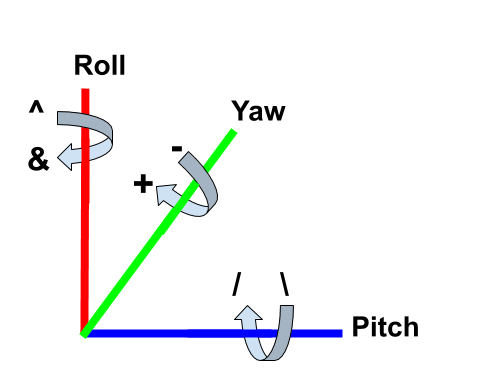
\includegraphics[scale=0.3]{Diagrams/rotations.png}
		}
		\caption{Diagram of the 3D rotations of the turtle.} \label{3D turtle rotations}
	}
\end{figure}
\FloatBarrier

\noindent
The turtle instructions are presented in such a way that allows movement in three dimensions. The rotations are represented as yaw, pitch and roll. Where yaw is a rotation around the Z axis, pitch is rotation around the X axis and roll is rotation around the Y axis. There are two symbols for each rotation, which represent positive and negative rotations respectively. Rotations are expected to be applied before a translation, that way the rotations change the orientation of the turtle and then the forward instructions move the turtle in the Y direction using the current orientation. The orientation is maintained from one translation to the next, and subsequent rotations are concatenated together to create a global orientation, in this way when the turtle moves forward again, it will move in the direction of this global orientation. Figure \ref{3D turtle rotations} shows the yaw, pitch and roll rotations as well as their axis and the instruction symbols for the L-system.\\
\\
The turtle instructions in the table \ref{DOL-system instructions}, can be used as the alphabet for the rewriting system defined in the L-system grammar below:

\begin{equation} \label{DOL-system example}
\begin{aligned}
	&\text{Generations: 1}\\
	&\text{Angle: 90$^{\circ}$}\\
	&\omega~~ : F \\
	&p_1~ :  F~ \rightarrow~ F+F-F-F+F\\
\end{aligned}
\end{equation}

\noindent
This L-system makes use of the alphabet "F, +, -". The meaning of these symbols is not relevent to the rewriting system. The main piece of information that is relevant to the interpreter is the angle to rotate by when it comes across the symbols + and -. This value is specified in the definition of the L-system with the Angle: 90$^{\circ}$ statement. The resulting string would be "F+F-F-F+F", this string is passed to the interpreter system which uses turtle graphics to execute the list of instructions. These instructions can be articulated in table \ref{Instruction Interpretation} below.

\begin{table}[h!]
\centering
\begin{tabular}{ | c | c | l | }
\hline
	 	Instruction Number & Instruction Symbol & Instruction Interpretation \\  
\hline
\hline
	I1 						& F & Move forward by 1\\
\hline
	I2						& + & Yaw right by 90 degrees\\
\hline
	I3						& F & Move forward by 1\\
\hline
	I4						& - & Yaw left by 90 degrees \\
\hline
	I5						& F & Move forward by 1\\
\hline
	I6 						& - & Yaw left by 90 degrees \\
\hline
	I7 						& F & Move forward by 1\\
\hline
	I8 						& + & Yaw right by 90 degrees\\
\hline
	I9 						& F & Move forward by 1\\
\hline
\end{tabular}
\caption{Table showing each instruction symbols and their interpretation for the L-system \ref{DOL-system example}}
\label{Instruction Interpretation}
\end{table}
\FloatBarrier

\noindent
These instructions are carried out one after the other, moving the turtle around the screen in three dimensions. Tracing the structure which the 0L-system has generated, these instructions will generate the traced line shown in figure \ref{basic turtle} below.

\begin{figure}[htbp]
	{\centering
		\setlength{\fboxrule}{1pt}
		\vspace{7px}
		\fbox{
			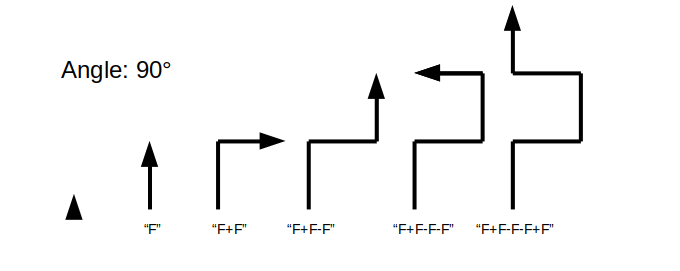
\includegraphics[scale=0.3]{Diagrams/basic_turtle.png}
		}
		\caption{Diagram showing a turtle interpreting simple L-system string.} \label{basic turtle}
	}
\end{figure}
\FloatBarrier

\noindent
As we can see from the turtle interpretation above, the turtle moves around as if it is an entity within a 3D world following a set of instructions that tell it where to move. This is the basic concept of turtle graphics and how it is implemented in the interpreter system. What also becomes apparent is that there are several assumptions which the interpreter makes in order to produce the final image in I9. It is assumed that that the + and - symbols mean a change in yaw of 90 degrees, and the second assumption is that the F symbol means to move forward by a distance of 1 unit measurement. The angle and distance values are assumed because the resultant string does not explicitly define the angle or the distance, it leaves that up to the interpretation of the string. 

In a simple DOL-system like the one above, there is no explicit way of providing this additional information to the interpreter. This means that it must be hardcoded into the interpretation or assumed by some other means. This highlights one of the main considerations when creating an L-system. There is a difference in complexities between the L-system rewriter and the interpreter. It is possible to create a very complex rewriting system with extensive rule systems, which can supply a large amount of information to the interpreter. The interpreter on the other hand can be rudimentary and follow the instructions exactly. Conversely, we could have a system where the L-system rewriter is quite basic, but the interpreter is very complex. The interpreter must be capable of representing the L-system, despite the lack of information in the resultant string, alternatively it should be able to obtain this information by other means. 

It may be tempting to leave the complexity to the interpreter in order to make the L-system rewriter and its rules more simple. However, the drawback of this, is that the information needed for modeling branch diameters, branching angles and even the type of objects that need to be rendered have to be supplied to the interpreter in some way. If not through the resulting string of information, how is this information meant to provided to the interpreter. An answer may be to build a system within the interpreter that is capable of assuming the general look of a plant, for instance, branches which decrement in diameter and branching angles which are consistant. This could results in a very inflexible system which may work for a portion of plant-life but might struggle to represent certain classes of plant-life. Therefore, the benefit of using a system with most of its complexity within the rewriting system is the L-system is responsible for some of the details of the interpretation such as angles, branch diameters and so on. In the next few sections, different types of L-systems will be discribed, explaining their benefits and limitations, as well as developing a system intergrating these separate systems into a single L-system grammar.   

There are several well known fractal geometry patterns that have been explored. They are particularly interesting because of how they seemingly imitate nature \cite{mandelbrot1982fractal}. An example of this is the is with edge-rewriting patterns like the Koch curve and the Sierpi\'{n}ski gasket. The Koch curve can be represented using the L-system defined in \ref{KochSnowflake} below. This is an adaption of the Koch snowflake which can be generated by the 0L-system. It is important to note that as the number of rewrite generations increases the complexity of pattern becomes increasingly intricate.

\begin{figure}[htbp]
	\raggedright
	\textbf{\underline{Koch Curves:}} \\
	Generations: 2,3,4\\
	Angle: 90$^\circ$\\
	Distance: 1 cm\\
	$\omega$ : F \\
	$p1$ : F $\rightarrow$ F+F-F-F+F\\
	{\centering
		\vspace{7px}
		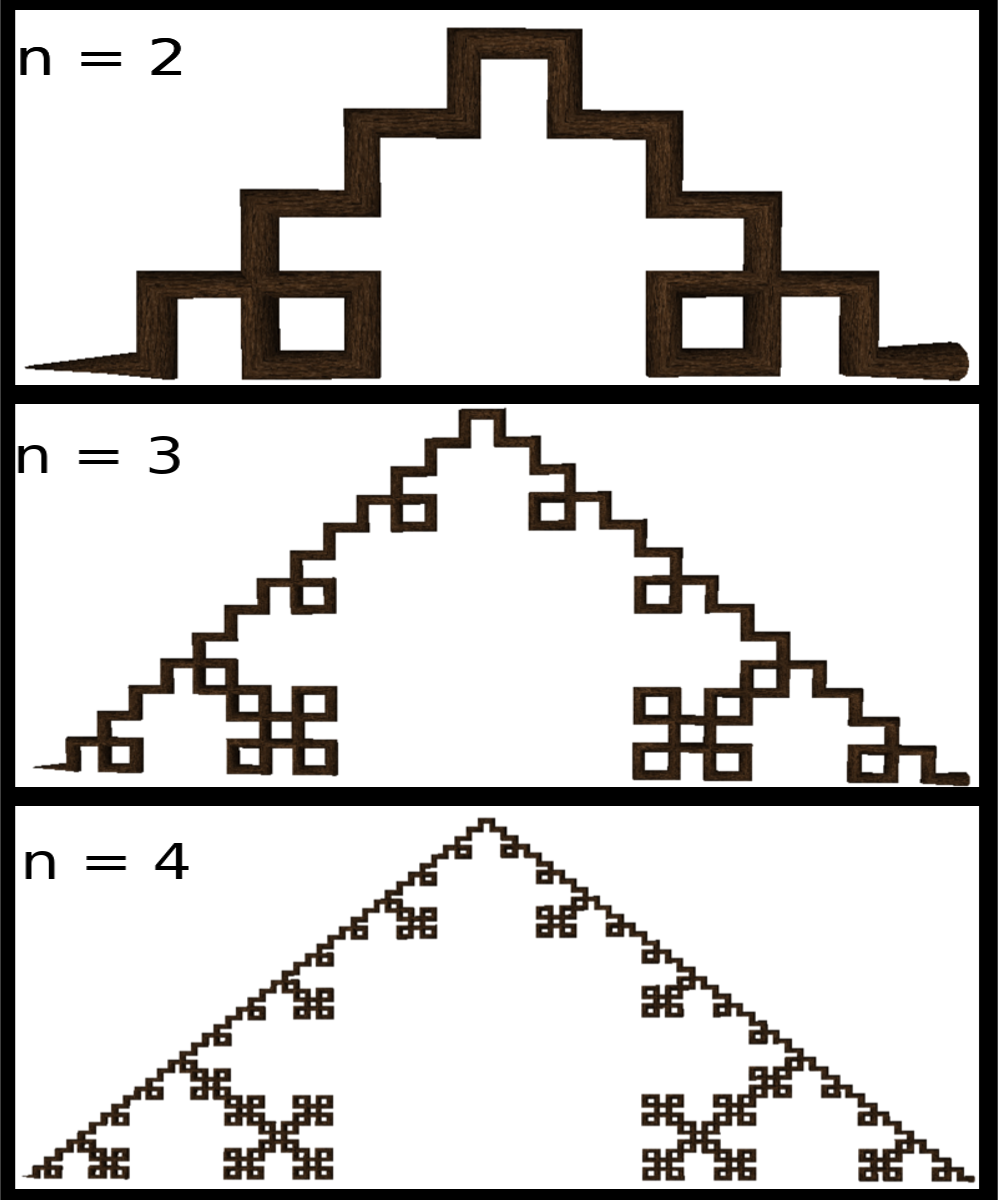
\includegraphics[scale=0.16]{Diagrams/koch_curves.png}
		\caption{Koch Curve.} \label{KochSnowflake}
	}
\end{figure}
\FloatBarrier

\noindent
The Sierpi\'{n}kski gasket is another example of an edge-rewriting pattern which can show the power of a rewriting system like the L-system. This example is interesting as with each generation the even numbered generations face left and the odd numbered generations face right.


\begin{figure}[htbp]
	\raggedright
	\textbf{\underline{Sierpi\'{n}ski Gasket:}} \\
	Generations: 2,3,4,5\\
	Angle: 60$^\circ$\\
	Distance: 1 cm\\
	$\omega$ : F\\
	$p1$ : F $\rightarrow$ X-F-X\\
	$p2$ : X $\rightarrow$ F+X+F\\
	{\centering
		\vspace{7px}
		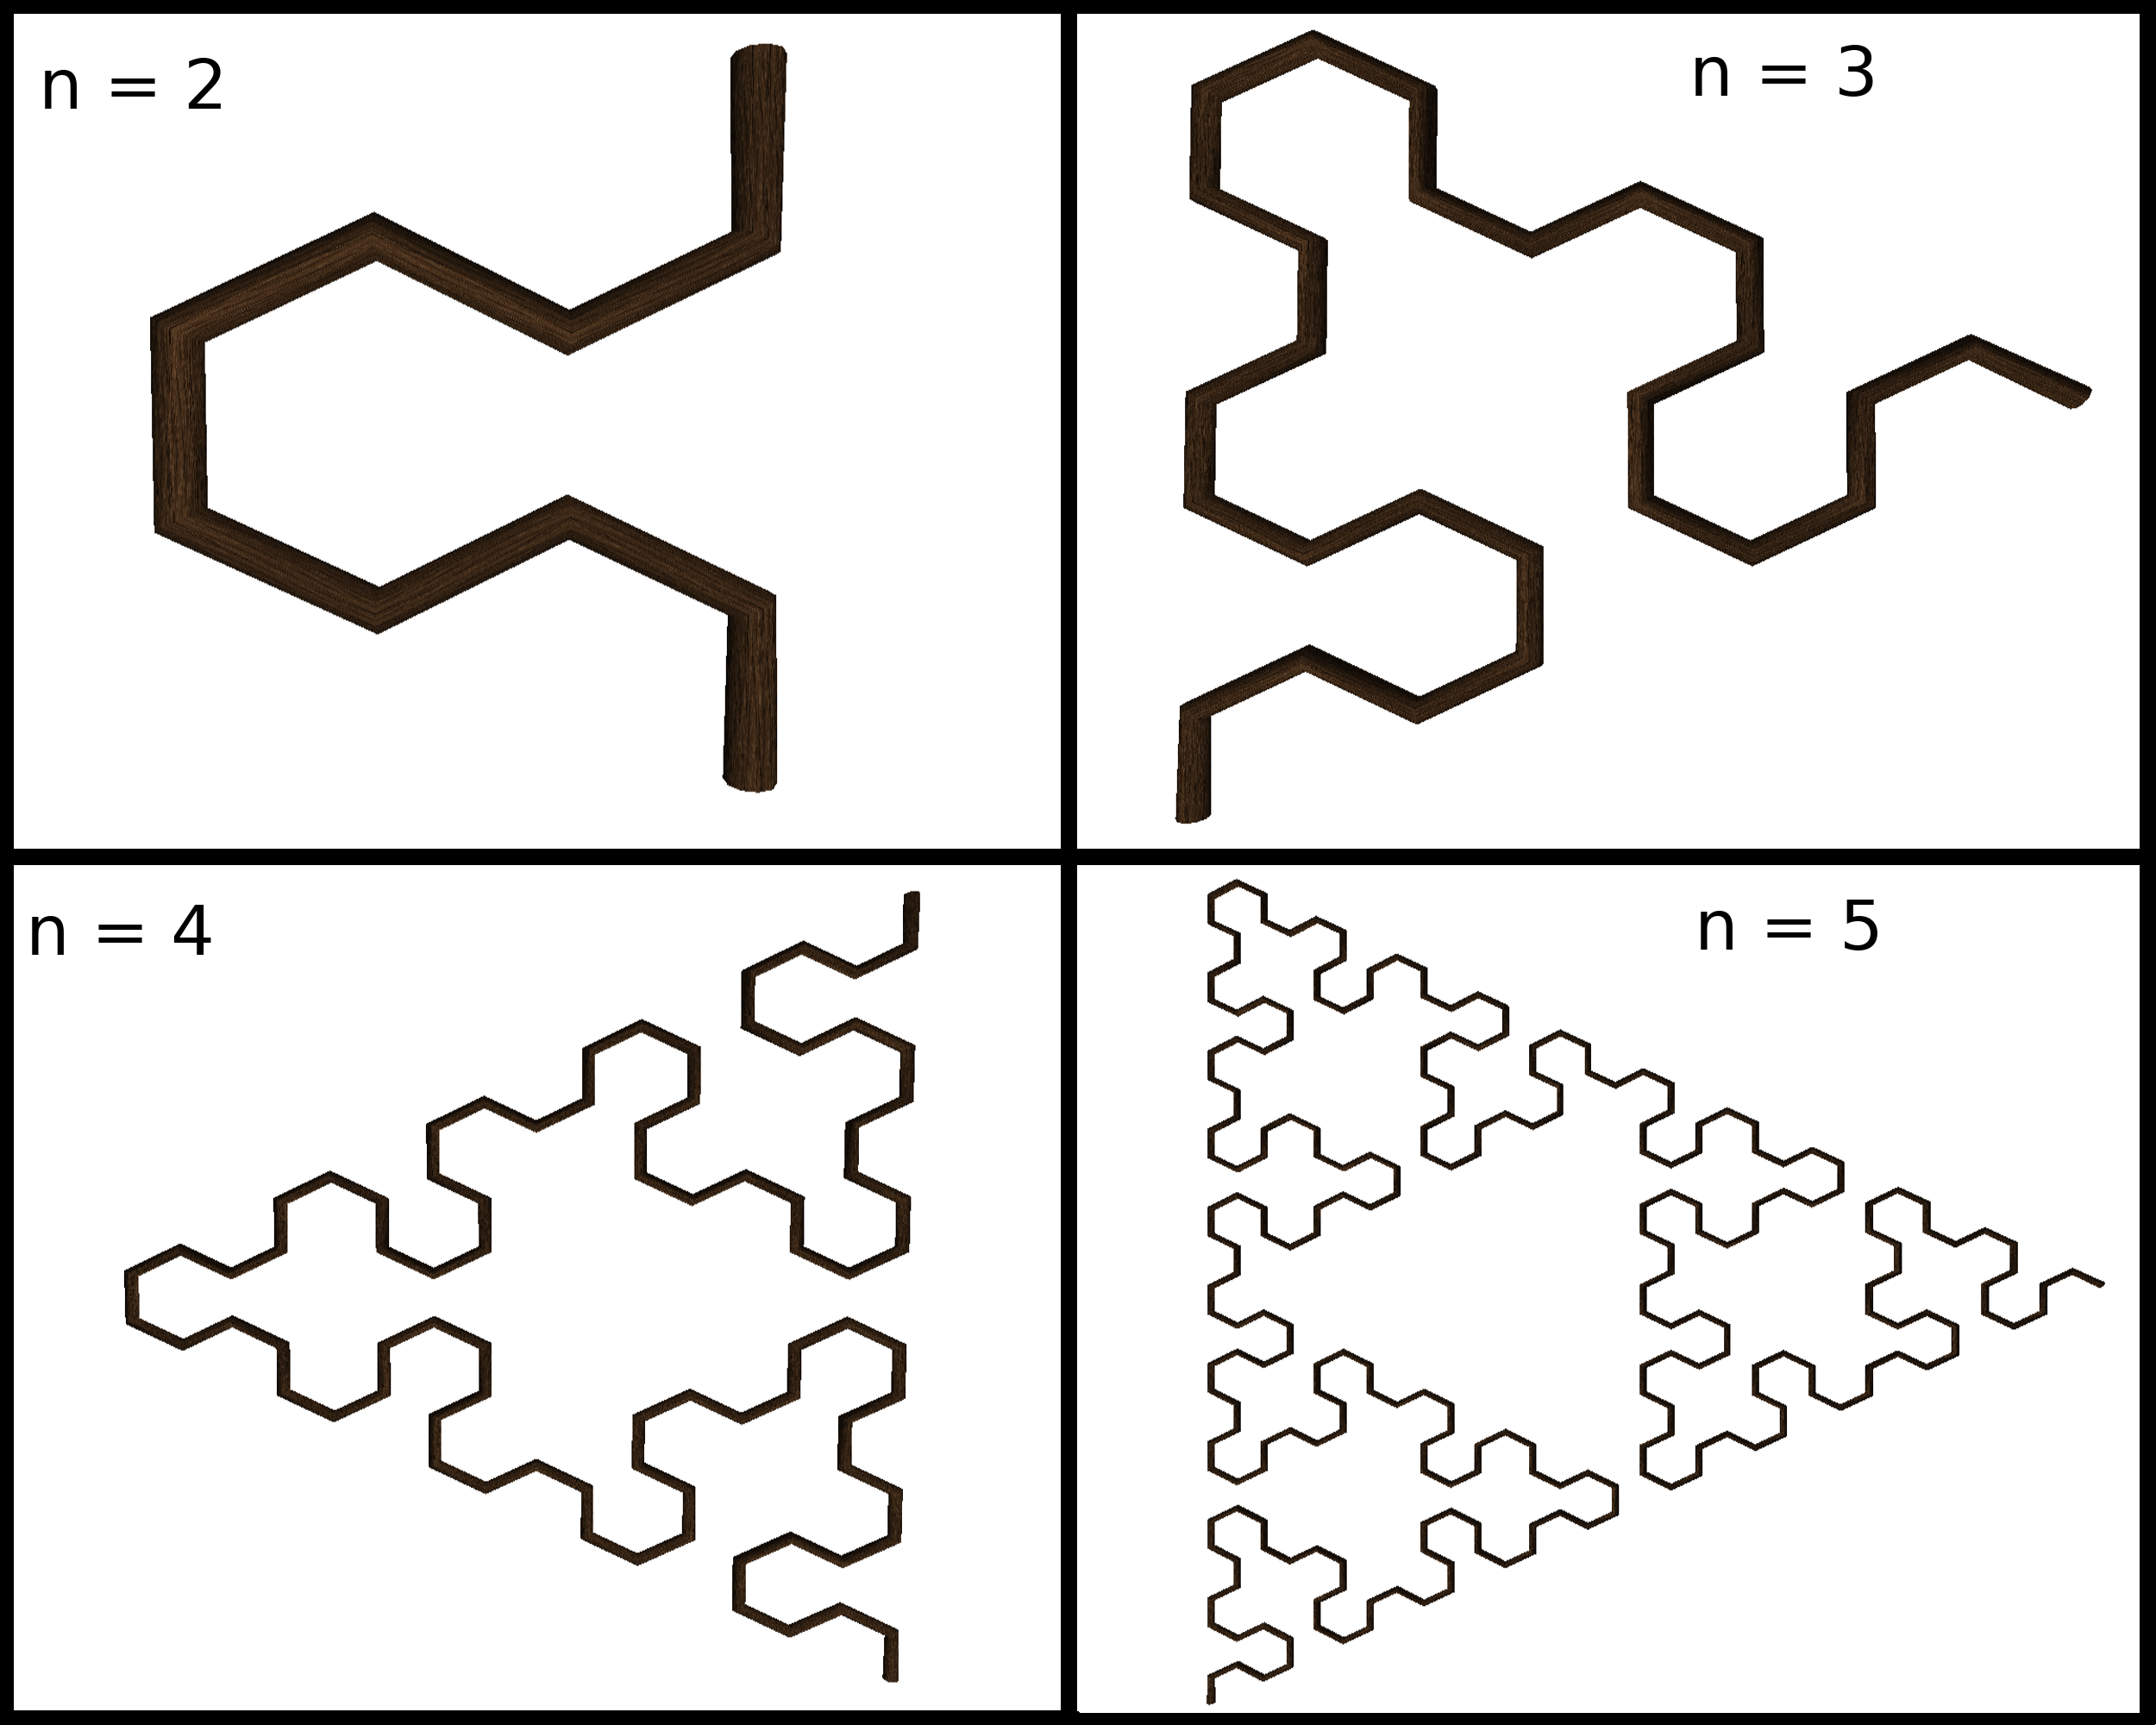
\includegraphics[scale=0.1]{Diagrams/sierpinsky_triangle.png}
		\caption{Sierpi\'{n}ski Triangles.}
	}
\end{figure}
\FloatBarrier

\section{Branching} \label{branching}

The simplistic D0L-system defined in previous sections can trace a 3D pattern. The D0L-systems interpretation provides a way of tracing a path or structure in 3D space. This is useful, however in order to trace the branching structure of plants, there needs to be a way of going to a point in the plant and branching off in one or more directions. A naive method may be for the turtle object to trace its steps back to a particular point and then branch off in a different direction. This may get the desired result but is slow and inefficient. A better solution was proposed by Lindenmayer. He introduced two symbols that have special meanings within the alphabet of the DOL-system which make branching much easier \cite{lindenmayer1968mathematical}. These are the square bracket symbols \say{[}, \say{]}. The open square bracket \say{[} symbol instructs the turtle object to save its current state (position and orientation) for the purpose of being able to go back to that saved state later. The close square bracket \say{]} instructs the turtle to load the saved state and continue from that position and orientation. This allows the turtle to jump back to a previously saved position, facing in the same direction as it was before. The orientation can be changed allowing the turtle to branch off in a different direction. This was originally used by Lindenmayer to develop the branching that occurs within algae but was later adapted by Smith to represent larger plant-life as well \cite{smith1984plants}.
 
The main advantage to using the save and load position functionality as a symbol within the alphabet is that the rewiting system itself handles branching. The production rules often contain the next generations branching structure by using the save and load symbols and thus the branching structure becomes more intricate from one generation to the next.

Each save state symbol must have a corresponding load state symbol within the string that is being interpreted. This is not a requirement by the L-system language but rather a requirement during by the interpreter. This is because the load and save state symbols have no special meaning when rewriting. It is simply treated the same as any other symbol in the alphabet. This being said, during interpretation, for the turtle object to jump back to a saved state those save and load states should correspond. For instance the resultant string \say{F[+F-F]-F} has both a load and a save state, meaning there is a single branch off the main branch. Which can be seen in figure \ref{branching 1} below. Additionally using nested save and load states in the string, for instance \say{F[+F[+F]-F]-F}, there can be two branches off the main branch twice as seen in figure \ref{branching 2}.

\begin{figure}[htbp]
	{\centering
		\setlength{\fboxrule}{1pt}
		\vspace{7px}
		\fbox{
			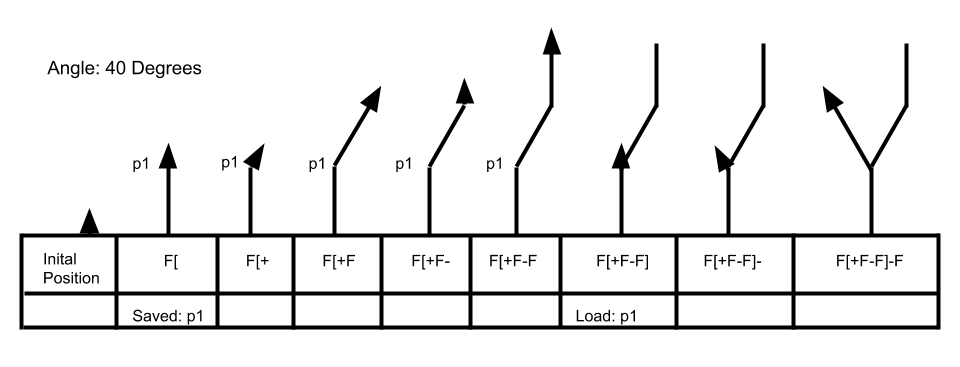
\includegraphics[scale=0.35]{Diagrams/branching.png}
		}
		\caption{Diagram showing a turtle interpreting an L-system using the branching symbols.} \label{branching 1}
	}
\end{figure}
\FloatBarrier

\noindent
Save and load operations are handled using the \acrfull{lifo} principle, meaning that when the save symbol is used the current position and orientation at $p1$ is saved. The next load state will restore $p1$'s position and orientation. Unless there is another save that takes place befoe the load state is reached, in which case the most recent save will have to be loaded before $p1$ can be loaded. In this way, the position saves are stacked and the most recent save is always loaded first. An example of this can be seen in figure \ref{branching 2} below:

\begin{figure}[htbp]
	{\centering
		\setlength{\fboxrule}{1pt}
		\vspace{7px}
		\fbox{
			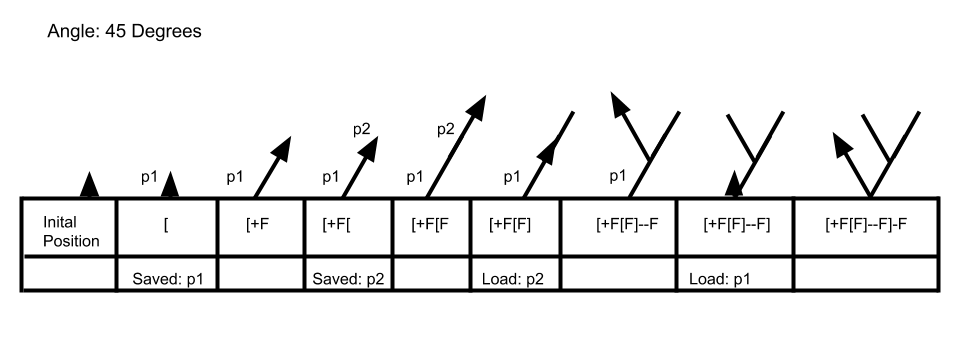
\includegraphics[scale=0.35]{Diagrams/NestedBranching.png}
		}
		\caption{Diagram showing a turtle interpreting an L-system with nested branching.} \label{branching 2}
	}
\end{figure}
\FloatBarrier

\noindent
The save and load state symbols can be used within a simple L-systems to create a more complex plant-like fractal pattern. In the examples below there are two different L-systems, one that is able to generate a fractal pattern similar to that of a bush and the other that is similar to a tree. In figure \ref{fractal bush} the F symbol can be rendered as a branch segment. The L-system only consists of a single rewriting rule thus each generation will result in exponentially more branches. In fact each generation results in eight times more branches than the previous generation. 

\begin{figure}[htbp]
	\raggedright
	\textbf{\underline{Fractal Bush:}} \\
	\textbf{Alphabet:} F, +, -, [, ] \\
	\textbf{Axiom:} F \\
	\textbf{Angle:} 25$^\circ$ \\
	\textbf{Rules:} \\
	F $\rightarrow$ FF+[+F-F-F]-[-F+F+F]\\
	{\centering
		\vspace{7px}
		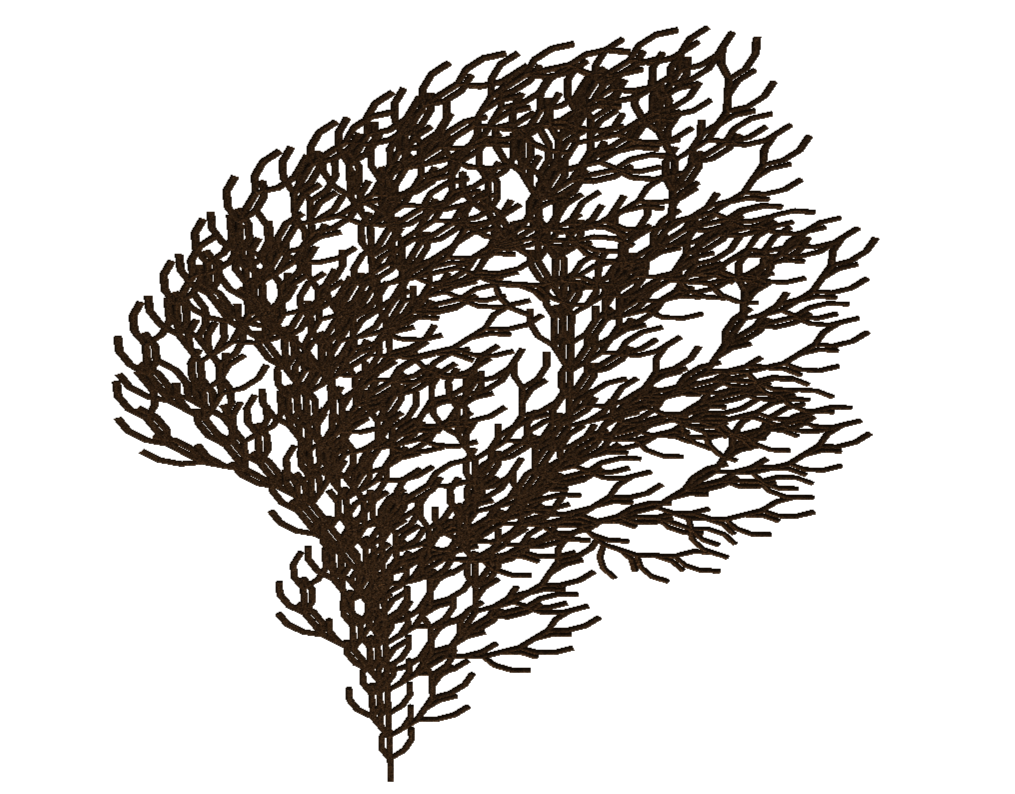
\includegraphics[scale=0.15]{Diagrams/fractalBush.png}
		\caption{Fifth generation of the fractal bush L-system.} \label{fractal bush}
	}
\end{figure}
\FloatBarrier

\noindent
In figure \ref{fractal plant} below, there are two different rewriting rules. One for the symbol F and the other for symbol X. Symbol X is the axiom, however, it is not a rendered symbol meaning it is ignored by the interpreter. Unlike the symbol F, which is rendered as a branch. Instead symbol X stands as a placeholder for the next rewriting step where it is rewritten with \say{F-[[X]+X]+F[+FX]-X}. The symbol F is simply replaced by FF, this means that existing branches will get longer each generation but new branching structures will be created at the end \say{leaves} or ends of the branches due to the production rule for symbol X.  

\begin{figure}[htbp]
	\raggedright
	\textbf{\underline{Fractal tree:}} \\
	\textbf{Alphabet:} X, F, +, -, [, ] \\
	\textbf{Axiom:} X \\
	\textbf{Angle:} 25$^\circ$ \\
	\textbf{Rules:} \\
	X $\rightarrow$ F-[[X]+X]+F[+FX]-X\\
	F $\rightarrow$ FF \\
	{\centering
		\vspace{7px}
		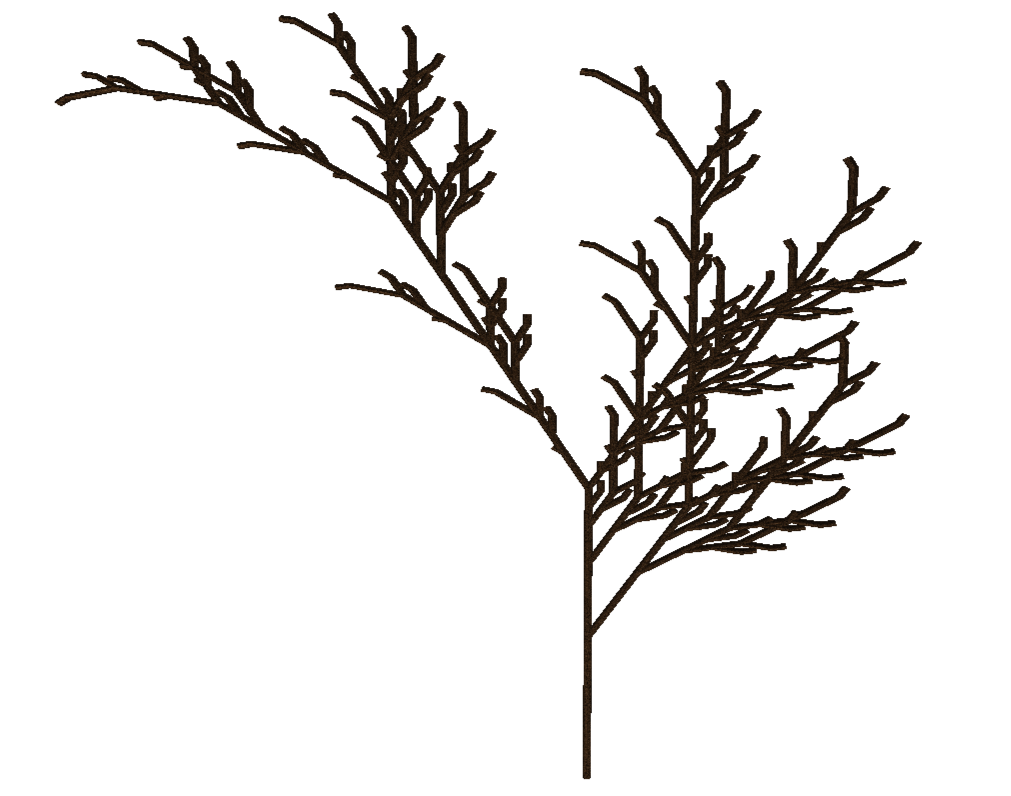
\includegraphics[scale=0.15]{Diagrams/fractalPlant.png}
		\caption{Fifth generation of the fractal tree L-system} \label{fractal plant}
	}
\end{figure}
\FloatBarrier

\section{Parametric OL-systems} \label{parametric}

Simplistic L-systems like the algae representation in section \ref{Simple DOL-systems} above, give us enough information to create a very basic structure of plant life, there are many details that are not included which a simple OL-system will not be able to represent. With the simplistic approach we have assumed that the width and length and branching angles of each section is constant or predefined. The result of this was that all of the details such as width and length of branches is left up to the interpretation of the resultant L-system string. This begs the question as to how we should accurately interpret the L-system string when we are not provided the details by the L-system. The answer lies in parametric 0L-systems.

In this section I will outline the definition and major concepts of the parametric L-system formulated by Prusinkiewicz and Hanan in 1990 \cite{prusinkiewicz1990visualization}, and developed upon in 2012 by Prusinkiewicz and Lindenmayer \cite{prusinkiewicz2012algorithmic}. I will also be talking about some of the changes that I have made, and explaining why these changes are necessary for the purpose of this thesis.


\subsection{Formal Definition of a Parametric 0L-system} \label{definition of a parametric 0L-system section}

Prusinkiewicz and Hanan define the parametric 0L-systems as a system of parametric words, where a string of letters make up a module name $A$, each module has a number of parameters associated with it. The module names belong an alphabet $V$, therefore, $A~ \in~ V$, and the parameters belong to a set of real numbers $\Re$. If $(a_1,~ a_2,~ ...,~ a_n)~ \in~ R$ are parameters of $A$, the module can be stated as $A(a_1,~ a_2,~ ...,~ a_n)$. Each module is an element of the set of modules $M~ =~ V~ \times~ \Re^*$. $\Re^*$ represents the set of all finite sequences of parameters, including the case where there are no parameters. We can then infer that $M^*~ =~ (V~ \times~ \Re^*)^*$ where $M^*$ is the set of all finite modules. 

Each parameter of a given module corresponds to a formal definition of that parameter defined within the L-system productions. Let the formal definition of a parameter be $\Sigma$. $ E(\Sigma) $ can be said to be an arithmetic expression of a given parameter.\\ Similar to the arithmetic expressions in the programming languages C/C++, we can make use of the arithmetic operators $ +,~ -,~ *,~ \,~ \wedge{}$. Furthermore, we can have a relational expression $C(\Sigma)$, with a set of relational operators. In the literature by Prusinkiewicz and Hanan the set of relational operators is said to be $<,~ >,~ =$, I have extended this to include the relational operators $>,~ <,~ >=,~ <=,~ ==,~ !=$. Where $==$ is the 'equal to' operator and $!=$ is the 'not equal' operator, and the symbols $>=$ and $<=$ are 'greater than or equal to' and 'less than or equal to' respectively. The parentheses () are also used in order to specify precedence within an expression. A set of arithmetic expressions can be said to be $\hat{E} (\Sigma)$,  these arithmetic expressions can be evaluated and will result in the real number parameter $\Re $, and the relational expressions can be evaluated to either true or false. \\
\\
The parametric 0L-system can be shown as follows as per Prusinkiewicz and Hanan's definition:

\begin{equation}
G~ = (V, \Sigma, \omega, P)
\end{equation}
\vspace{5mm}

\noindent
$G$ is an ordererd quadruplet that describes the parametric OL-system. $V$ is the alphabet of characters for the system. $\Sigma$ is the set of formal parameters for the system. $\omega~ \in~ (V~ \times \Re^*)^+$ is a non-empty parametric word called the axiom. Finally $P$ is a finite set of production rules which can be fully defined as:

\begin{equation}
P~ \subset~ (V~ \times~ \Sigma^*)~ \times C(\Sigma)~ \times~ (V~ \times~ \hat{E}(\Sigma))^*
\end{equation}

\noindent
Where $(V~ \times~ \Sigma^*) $ is the predecessor module, $C(\Sigma) $ is the condition and $(V~ \times~ E(\Sigma))^* $ is the set of successor modules. For the sake of readability we can write out a production rule as \textit{predecessor} : \textit{condition} $\rightarrow$ \textit{successor}. I will be explaining the use of conditions in production rules in more detail in section \ref{Condition L-system Subsection}.
A module is said to match a production rule predecessor if they meet the three criteria below.

\begin{itemize}
\item The name of the axiom module matches the name of the production predecessor.
\item The number of parameters for the axiom module is the same as the number of parameters for the production predecessor.
\item The condition of the production evaluates to true. If there is no condition, then the result is true by default.
\end{itemize}

\noindent
In the case where the module does not match any of the production rule predecessors, the module is left unchanged, effectively rewriting itself. 


\subsection{Defining Constants and Objects}

There are some other features covered by Prusinkiewicz and Lindenmayer, that are not specific to the parametric L-systems definition itself but serve more as quality of life. In the literature, they refer to the \#define which is said "To assign values to numerical constants used in the L-system" as well as the \#include statement which specifies what type of shape to draw by refering to a library of predefined shapes \cite{prusinkiewicz2012algorithmic}.
\noindent
For instance if we have an value for an angle that we would like to use within the production rules we can use the \#define statement as follows:

\begin{equation} \label{define statement example}
\begin{aligned}
	&n=4 \\
	&\textrm{\#define angle 90}\\
	&\omega~~ : F(5)\\
	&p_1~ :  F(x)~~~~~ :~ * \rightarrow~ F(w)+(angle)F(w)+(angle)F(w)+(angle)F(w)\\
\end{aligned}
\end{equation}

Here you can see that the \#define acts like a declaration, where we are going to be defining a variable which will be used later. Essentially we are replacing any occurences of the variable \textit{angle} with the value of 90 degrees. The define statement is written as  \#define \textit{variable\_name} \textit{value}.

With regards to the \#include statement, In the literature the \#include may be used by stating \say{\#include H}. This would tell the turtle interpreter that the symbol \say{H} is a shape in a library of predefined shapes which should be rendered instead of the default shape. This functionality has been slightly modified, instead of the \#include statement, the \#object is used and serves a similar purpose, however, instead importing the symbol \say{H}, denoting to the hetrocist object from a library of predefined shapes, The statement \say{\#object H HETEROCYST} specifies that we are associating the symbol or module \say{H} with the object HETEROCYST. The HETEROCYST object is still stored in a predefined library, however, the advantage is that the object can be associated with multiple different symbols, it also does not limit us to a predefined name for an object. Below is an example using the \#object statement: 

\begin{equation} \label{object statement example}
\begin{aligned}
	&n=1 \\
	&\textrm{\#object F BRANCH}\\
	&\textrm{\#object S SPHERE}\\
	&\omega~~ : F(1)\\
	&p_1~ :  F(x)~~~~~ :~ * \rightarrow~ F(w)F(w)F(w)F(w)S(w)\\
\end{aligned}
\end{equation}

\begin{figure}[htbp]
	{\centering
		\vspace{7px}
		\setlength{\fboxrule}{1pt}
		\fbox{
			
\includegraphics[scale=0.2]{Diagrams/object_example.png}
		}
		\caption{Diagram of an L-system Using Multiple Objects.}
	}
\end{figure}
\FloatBarrier

\noindent
In the simple example in figure \ref{object statement example} above, you can see that the first three F modules render a branch segment with length of 1.0, however, for the final S module renders a sphere of diameter 1.0. The geometric shape that is eventually rendered does not affect the L-system in any way and the \#object feature bares no meaning to the rewriting system, it simply stands as an instruction to the interpreter which instructs that each time the symbols F or S are interpreted, a specific object should be rendered, such as BRANCH and SPHERE respectively. The position of the next object or branch can then be determined by moving forward by the diameter of the object and rendering the next object from that point, this will be discussed more detail chapter \ref{interpreter implementation} where the turtle graphics interpreter and renderer is defined.

\subsection{Modules With Special Meanings}

In the above section I defined the details of a parametric 0L-system, in the paper by Prusinkiewicz and Lindenmayer, there are two operators which I have not discussed yet, those are the ! and the ‘. Prusinkiewicz and Lindenmayer state that “The symbols ! and ‘ are used to decrement the diameter of segments and increment the current index to the color table respectively” \cite{prusinkiewicz2012algorithmic}. We have decided to modify this to work slightly differently, the ! and ‘ will still perform the same operation, however the ! and ‘ symbols are actually treated as a module that holds a particular meaning to the interpreter, rather than a single operator, furthermore, they share the same properties with modules, they can contain multiple parameters, and depending on the number of parameters they can be treated differently. The module ! with no parameters could mean decrement the diameter of the segment by a default amount, whereas !(10) means set the diameter of the segment to 10. The length can also be manipulated in a similar manner. The module with the name F has a default meaning to create a segment in the current direction by a default amount. If we provide the module F(10) we are specifying to create a segment of length 10.

Using the L-system below we can create figure \ref{parametric l-system practical}, the concepts discussed above have been used by decrementing the segment diameter during the rewriting process as well as by incrementing the branch length.

\begin{equation} \label{parametric l-system practical}
\begin{aligned}
	&n=8 \\
	&\omega~~ : A(5)\\
	&p_1~ :  A(w)~~~~~ :~ * \rightarrow~ F(1)!(w)[+A(w~*~0.707)][-A(w~*~0.707)]\\
	&p_2~ :  F(s)~~~~~ :~ * \rightarrow~ F(s~*~1.456)\\
\end{aligned}
\end{equation}

The above l-system gives the resulting representation shown below in figure 3.8. 

\begin{figure}[htbp]
	{\centering
		\vspace{7px}
		\setlength{\fboxrule}{1pt}
		\fbox{
			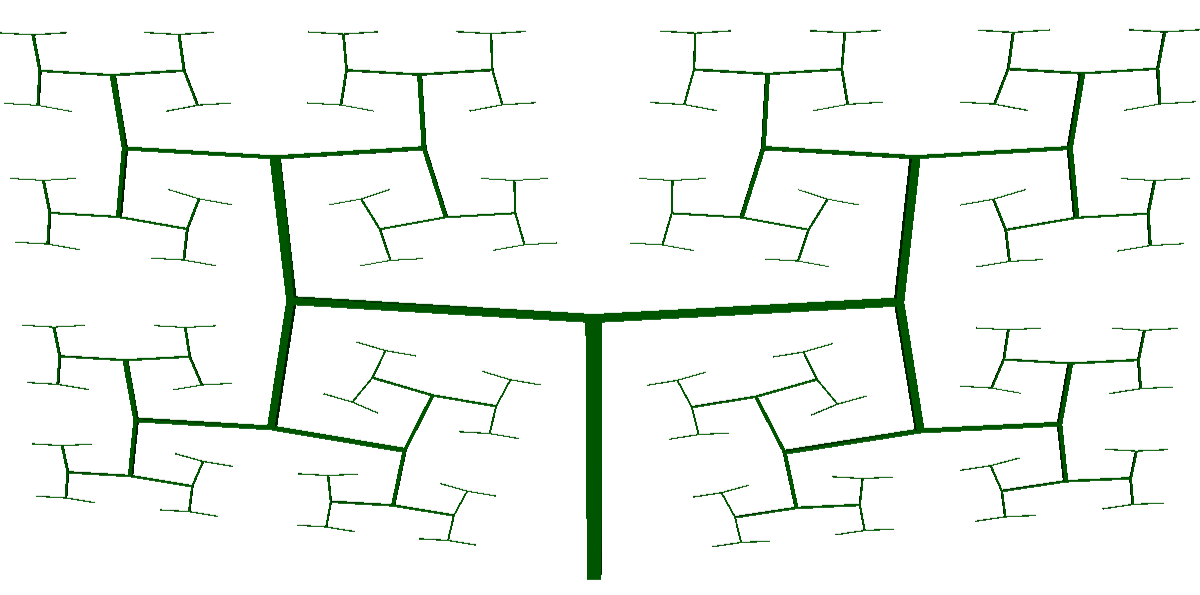
\includegraphics[scale=0.30]{ParametricLsystem/branchingPattern.png}
		}
		\caption{3D Parametric L-system.}
	}
\end{figure}
\FloatBarrier

\noindent
This gives a much more realistic looking tree structure as the branch segments become shorter but also become thinner in diameter as they get closer to the end of the branch as a whole. 

\subsection{Representing L-system Conditions} \label{Condition L-system Subsection}

A condition allows us to have multiple production rules that are the same in terms of the module name and the number of parameters that they have, furthermore, they require a particular condition to be met in order for the module to match that rule. 

In this section I will be detailing the use of the condition statement, which lies between the predecessor and the successor in a production rule, and can be seen as an a mathematical expression on either side of a relational operator. During the rule selection process the expressions are evaluated and the results are compared using the condition operator. If the result of the condition is true then that rule is selected for rewriting, if the result is false then it moves on to check the next rule. 


Below is an example of a parametric 0L-system using condition statements:

\begin{equation} \label{parametric l-system example}
\begin{aligned}
	&n=5 \\
	&\omega~~ : A(0)B(0,4)\\
	&p_1~ :  A(x)~~~~~ :~ x~ >~ 2~ \rightarrow~ C\\
	&p_2~ :  A(x)~~~~~ :~ x~ <~ 2~ \rightarrow~ A(x~ +~ 1)\\
	&p_3~ :  B(x,~ y)~ :~ x~ >~ y~ \rightarrow~ D\\
	&p_4~ :  B(x,~ y)~ :~ x~ <~ y~ \rightarrow~ B(x~ +~ 1,~ y)\\
\end{aligned}
\end{equation}

\noindent
The L-system above in \ref{parametric l-system example} is rewritten five times using the axiom specified by the symbol $\omega$, as well as the four production rules $p_1, p_2, p_3, p_4$. Each generation of the rewritting process can be seen below in \ref{parametric l-system example result}.

\begin{equation} \label{parametric l-system example result}
\begin{aligned}
	&g_0 :~ A(0)B(0,~4)\\
	&g_1 :~ A(1)B(1,~4)\\
	&g_2 :~ A(2)B(2,~4)\\
	&g_3 :~ C~B(3,~4)\\
	&g_4 :~ C~B(4,~4)\\
	&g_5 :~ C~D\\
\end{aligned}
\end{equation}

\noindent
A practical use of the condition statement might be to simulate different stages of growth. This is best illustrated using the L-system below: 

\begin{equation} \label{conditional l-system example}
\begin{aligned}
	&n=2,~4,~6 \\
	&\#\text{object F BRANCH} \\
 	&\#\text{object L LEAF} \\
	&\#\text{object S SPHERE} \\
	&\#\text{define r 45} \\
	&\#\text{define len 0.5} \\
	&\#\text{define lean 5.0} \\
	&\#\text{define flowerW 1.0} \\
	&\omega~~ :~ !(0.1)I(5)\\
	&p_1~ :  I(x)~ :~ x~ >~ 0~~ \rightarrow~ F(len)-(lean)[R({0, 100})]F(len)[R({0, 100})]I(x-1)\\
	&p_2~ :  R(x)~ :~ x~ >~ 50~ \rightarrow~ -(r)/(20)!(2.0)L(2)!(0.1)\\
	&p_3~ :  R(x)~ :~ x~ <~ 50~ \rightarrow~ -(r)\backslash(170)!(2.0)L(2)!(0.1)\\
	&p_4~ :  I(x)~ :~ x~ <=~ 0~ \rightarrow~ F(len)!(flowerW)S(0.3)\\
\end{aligned}
\end{equation}

\begin{figure}[htbp]
	{\centering
		\vspace{7px}
		\setlength{\fboxrule}{1pt}
		\fbox{
			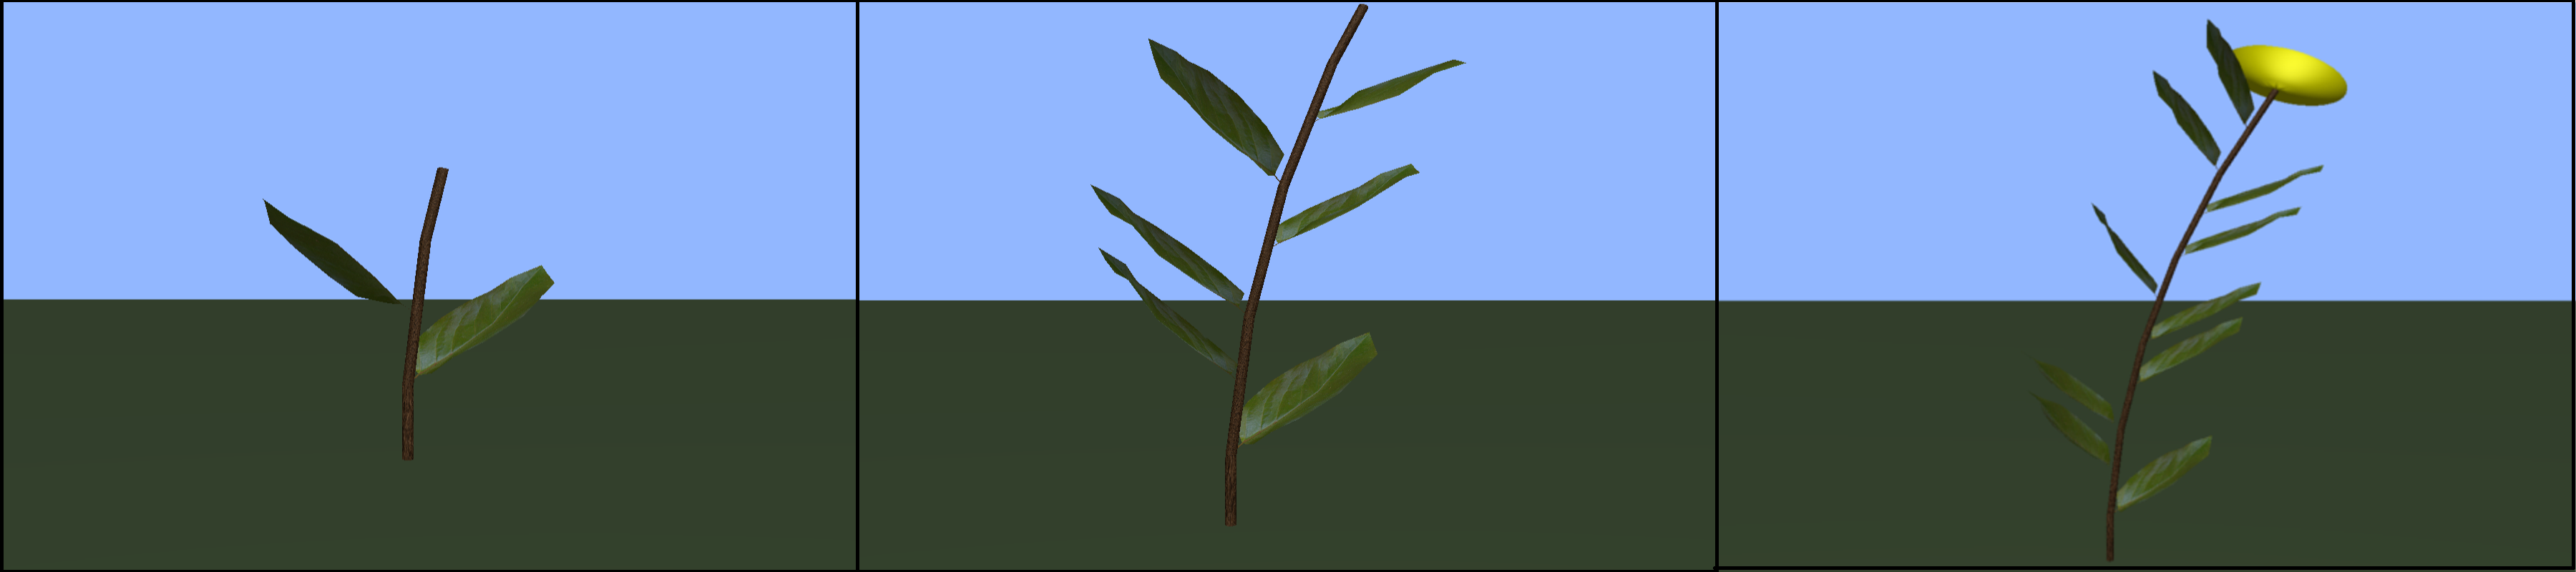
\includegraphics[scale=0.12]{Diagrams/conditionalLsystem.png}
		}
		\caption{Condition statements used to simulate the growth of a flower. 2nd generation on the left, 4th generation in the center and 6th generation on the right}
	}
\end{figure}
\FloatBarrier


\section{Randomness within L-systems} \label{Randomness L-system Subsection}

Randomness is an essential part of nature. If there was no randomness in plant life, it would end up with very symetric and unrealistic. Randomness is also responsible for creating variation in the same L-system. A L-system essentially describes the structure and species of a plant. It describes everything from how large the trunk of the tree is, to how many leaves there are on the end of branch, or even if it has flowers or not. However if there is no capability to have randomness in the generation of the L-system then we will always end up with the exact same structure. 
\vspace{5mm}
Below is a simple example of how randomness can be used to create variation.

\begin{equation} \label{randomness example}
\begin{aligned}
	&n=2\\
	&\text{\#define r 25} \\
	&\omega~~ :~ !(0.2)F(1.0)\\
	&p_1~ :  F(x)~ :~ *~ \rightarrow~ F(x)[+(r)F(x)][-(r)F(x)]+(\{-20, 20\})F(x)-(\{-20, 20\})F(x)\\
\end{aligned}
\end{equation}

\begin{figure}[htbp]

	{\centering
		\setlength{\fboxrule}{0pt}
		\fbox{
			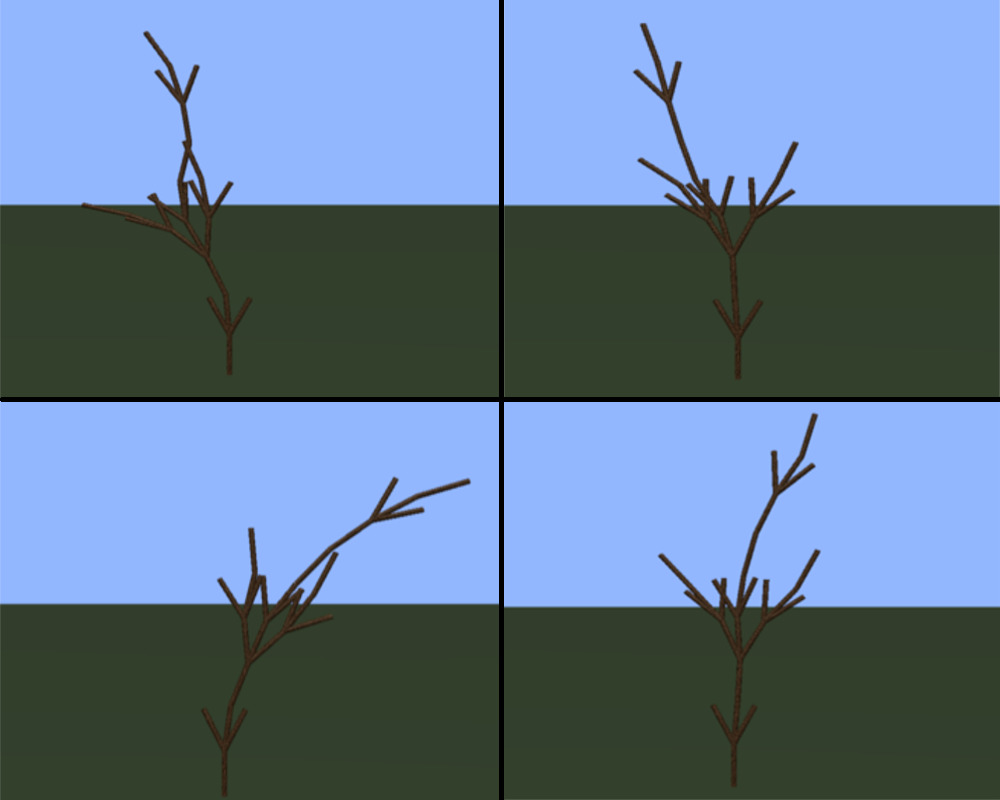
\includegraphics[scale=0.15]{Diagrams/RandomTrees.png}
		}
		\caption{Different Variations of the Same L-system with Randomness Introduced in The Angles. \label{figRandomness}}
	}
\end{figure}
\FloatBarrier

\noindent
In figure \ref{figRandomness} there are four variations of the same L-system using randomness, We can specify that we would like to create a random number by using the expression \{-20.0, 20.0\}. The curly braces signify that what is contained is a random number range, ranging from the minimum value as the first floating point value and the maximum value as the second floating point value separated by a comma. If both values are the same for instance +(\{10.0, 10.0\}) this is equivilant to +(10.0).

\section{Stochastic Rules within L-systems} \label{Stochastic L-system Subsection}

Similar to the previous section about randomness in L-systems, stochastic L-systems fulfill a similar goal. 0L-systems on their own are incapable of creating any variation, they simply follow a strict set of production rules which gives the same result. Introducing randomness to an 0L-system for width, length and other parameters can result in a plant that looks slightly different but does not change to overall structure of the plant or any branching. In order to create a different structure for a plant we must introduce stochastic probability within the selection of the production rules, thus effecting the rewriting of the structure itself.

Eichhorst and Savitch introduced a new type of 0L-system called the S0L-system, this added two features to the existing 0L-system, firstly the S0L-system is not limited to defining a single axiom (starting point), a finite number of starting points can be defined and a probability distribution is used in order to select the starting point at the start of the rewriting process. Secondly, the S0L-system allows you to define a finite number of production rules which have a probability distribution in order to decide which rule should be chosen for rewriting \cite{eichhorst1980growth}. Similarly an article by Yokomori proposes a stochastic 0L-system which also proposes a measure of the entropy of a string generated by a 0L-system \cite{yokomori1980stochastic}.\\
Later, Prusinkiewicz and Lindenmayer built upon this by creating a definition of a stochastic L-system, that makes use of the stochastic nature of the production rules from the SOL-system. In this paper, I will be using the definition of the stochastic 0L-system defined by Prusinkiewicz and Lindenmayer, and developing them into the existing parametric 0L-system. This paper will not allow multiple starting points as defined by Eichhorst and Savitch in the SOL-system, as it does not seem necessary and could overcomplicate the 0L-system, however, this functionality could be added in the future if it is seen to be neccessary. \\
Similarly to the 0L-sysstem, the stochastic 0L-system is an ordered quadruplet, represented as $G_\pi~ = (V, \omega, P, \pi)$, where $V$ is the alphabet of the 0L-system, $\omega$ is the axiom, $P$ is the finite set of productions and $\pi$ represents a probability distribution for a set of production probabilities this can be shown as $\pi~ :~ P~ \rightarrow~ (0, 1)$ the production probabilities must be between 0 and 1 and the sum of all production probabilies must add up to 1.

The following L-system definition created by Prusinkiewicz and Lindenmayer states three production rules with each rule having a probability of 0.33 out of one. For a finite set of production rules to be stochastic, the production rules must share the same module name an the same number of parameters. There must be two or more production rules and the total probability distribution must add up to 1.0 \cite{prusinkiewicz2012algorithmic}.

\begin{equation} \label{stochastic example}
\begin{aligned}
	&n=5\\
	&\text{\#define r 25}\\
	&\omega~~ :~ F(1)\\
	&p_1~ :  F(x)~ :~ \sim 0.33 ~ \rightarrow~ F(x)[+(r)F(x)]F(x)[-(r)F(x)]F(x)\\
	&p_2~ :  F(x)~ :~ \sim 0.33 ~ \rightarrow~ F(x)[+(r)F(x)]F(x)\\
	&p_3~ :  F(x)~ :~ \sim 0.34 ~ \rightarrow~ F(x)[-(r)F(x)]F(x)\\
\end{aligned}
\end{equation}

\noindent
As you can see the module F(x) above, is the predecessor for all three of the production rules, each rule has a probability which is defined using the $\sim$ symbol followed by probability from 0 to  1. In the above example each probability isapproximately one third, they are approximate in order to total a an exact probability of 1.0. During the rewriting process, when the module F with one parameter is found, a production rule is randomly selected using the probability distribution described within the production rule. The predecessor from the selected rule with then rewrite that module. 

\begin{figure}[htbp]
	{\centering
		\vspace{7px}
		\setlength{\fboxrule}{1pt}
		\fbox{
			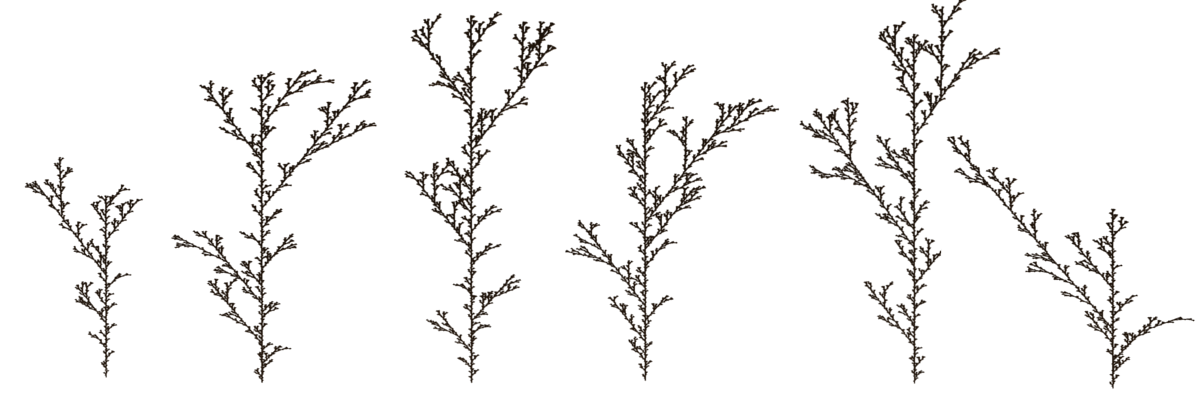
\includegraphics[scale=0.35]{Diagrams/stochastics.png}
		}
		\caption{Representation of an L-system with a probability stochastic with a 0.33 probabability for each rule.} \label{stochastic diagram}
	}
\end{figure}
\FloatBarrier

\noindent
The stochastic L-system definition in \ref{stochastic example}, produces the following fractal structures seen in figure \ref{stochastic diagram} below. The stochastic L-system will get a slightly different resultant string each time it is run, depending on which rules were selected for rewriting. This gives a different number of translation instructions, can result in the plants having branches of different lengths, for example $p1$ has two extra F instructions. Resulting in some branches being much longer than others, as well as possibly producing plants of different sizes. 

\begin{figure}[htbp]
	{\centering
		\setlength{\fboxrule}{1pt}
		\vspace{7px}
		\fbox{
			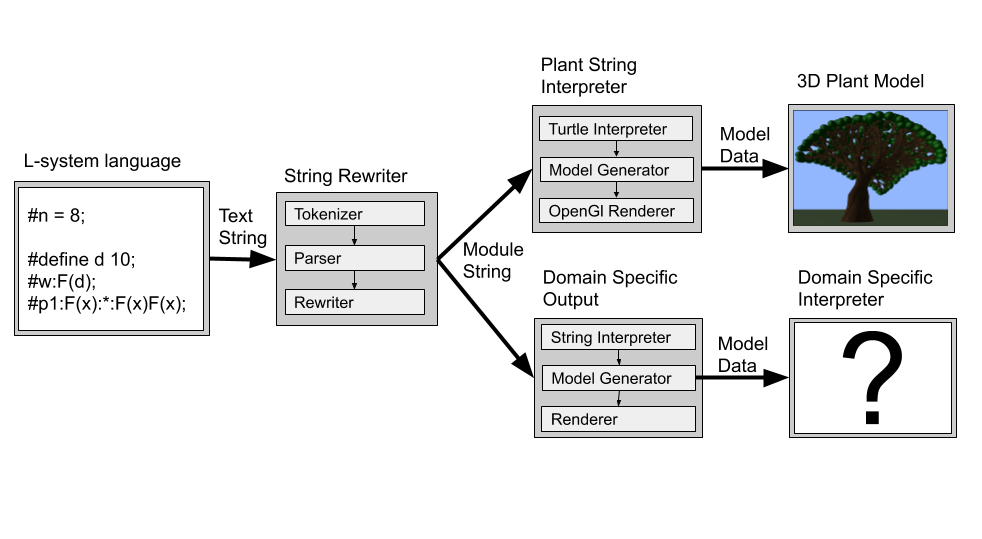
\includegraphics[scale=0.43]{Diagrams/FullDiagram.png}
			\label{3DAxisFigure}
		}
		\caption{Diagram of the procedural generation process.}
	}
\end{figure}
\FloatBarrier

\section{Summary}

L-systems represent a set of state transitions based upon the production rules provided, these rules dictate how a string will be rewritten, which in turn determines the overall structure of the plant it is trying to represent. The symbols in D0L-systems or modules in parametric 0L-systems represent particular instructions to be carried out by turtle graphics within the interpreter. The symbols or modules within an L-system do not change the behaviour of the L-system but matter only to the interpreter. Additionally the complexity of the L-system rewriter decides the complexity of the interpreter, if a L-system provides a large amount of information to the interpreter, less assumptions need to be made during the interpretation and therefore, providing the able to more accurately describe the plant-life it is representing.

By using the parametric 0L-system we can build in a number of features, otherwise used in other L-systems, such as branching, conditional production rules, randomness in parameters, stochasticity. These features allow the parametric 0L-system to represent plant-life with varying structures as well as branch lengths, branch widths and production rule conditions can give control over stages of growth.

